\documentclass{llncs}

\usepackage[usenames,dvipsnames]{color}
\usepackage{graphicx}

%%%%%%%%%%%%%%%%%%%%%%%%%%%%%%%%%%%%%%%%%%%%%%


% Allow comments by name
\renewcommand{\note}[2]{\textbf{\textcolor{#1}{#2}}}
\newcommand{\comment}[1]{\note{red}{#1}}
\newcommand{\dave}[1]{\note{PineGreen}{Dave: #1}}
\newcommand{\magda}[1]{\note{Cyan}{Magda: #1}}
\newcommand{\tom}[1]{\note{OrangeRed}{Tom: #1}}
% To remove all notes, uncomment the next line.
%\renewcommand{\note}[2]{\unskip}


% Figures
\newcommand{\figurerig}{
\begin{figure}[tbp]
  \centering
  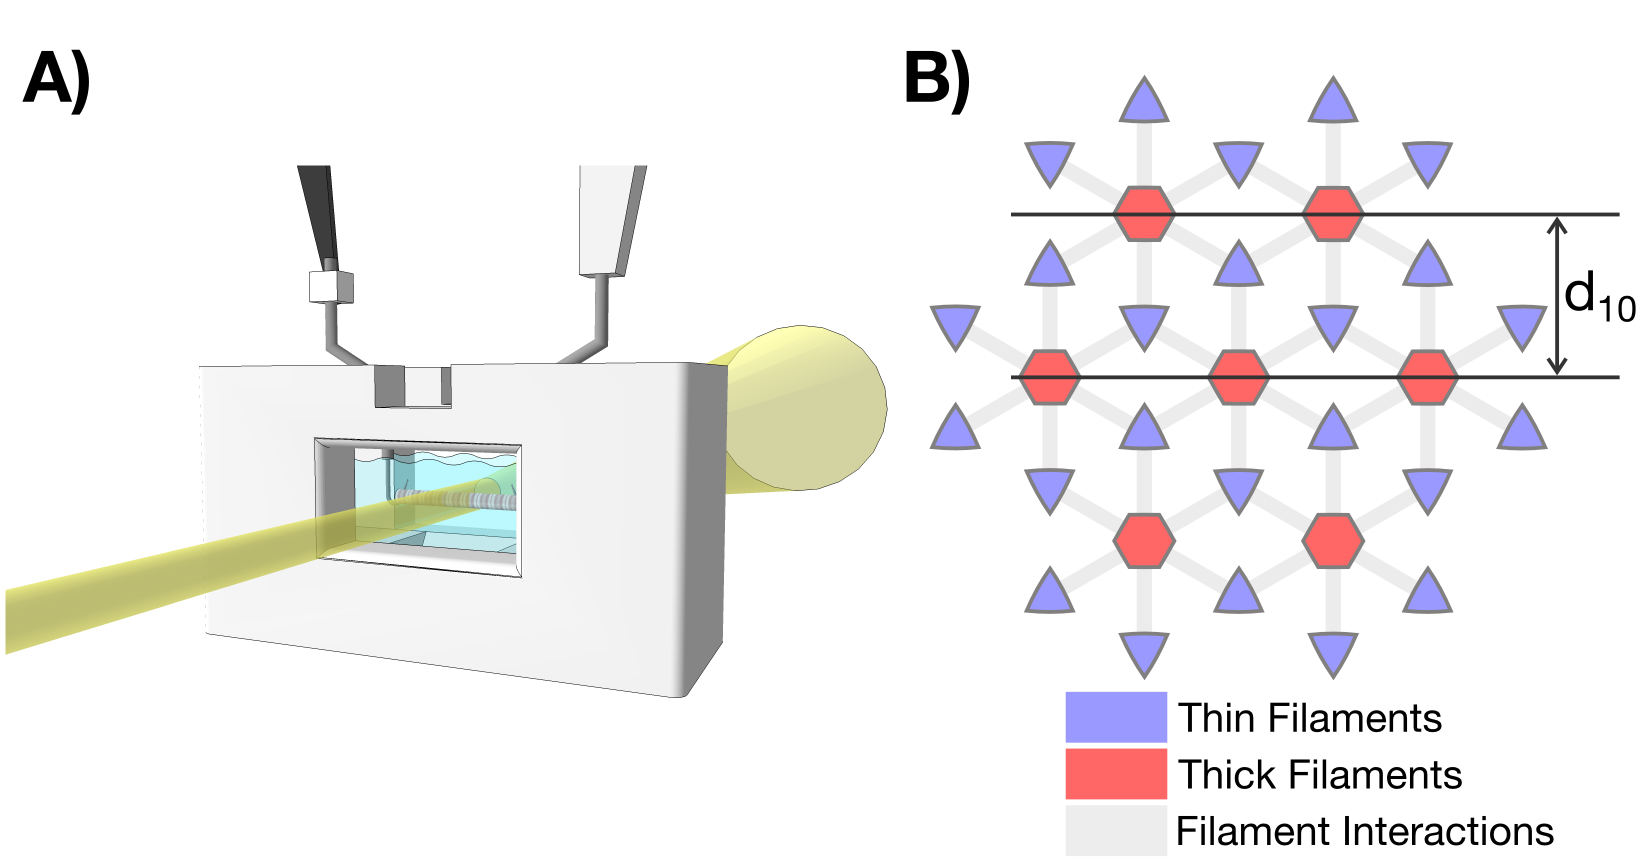
\includegraphics[width=.8\linewidth]{figures/rig_and_lattice}
  \caption{\label{fig:rig}
    Data collection and interpretation.  
    A) Diffractive imaging of an isolated muscle sample requires a
    physiological solution bath with top entry for mounting to
    force/length controllers (arms) and front and rear cut outs to
    allow the X-ray beam to pass through and scatter off the muscle
    sample. B) Muscle's contractile lattice is composed of thick and
    thin filaments. When viewed down the long axis, these filaments
    form a hexagonal array. The $d_{10}$ spacing is the distance
    between adjacent lines of thick filaments, and is proportional to
    the distance molecular motors (gray links) must diffuse across in
    order to bind. 
	}
	\vspace{-10pt}
\end{figure}
}

\newcommand{\figureimgs}{
\begin{figure}[tbp]
  \centering
  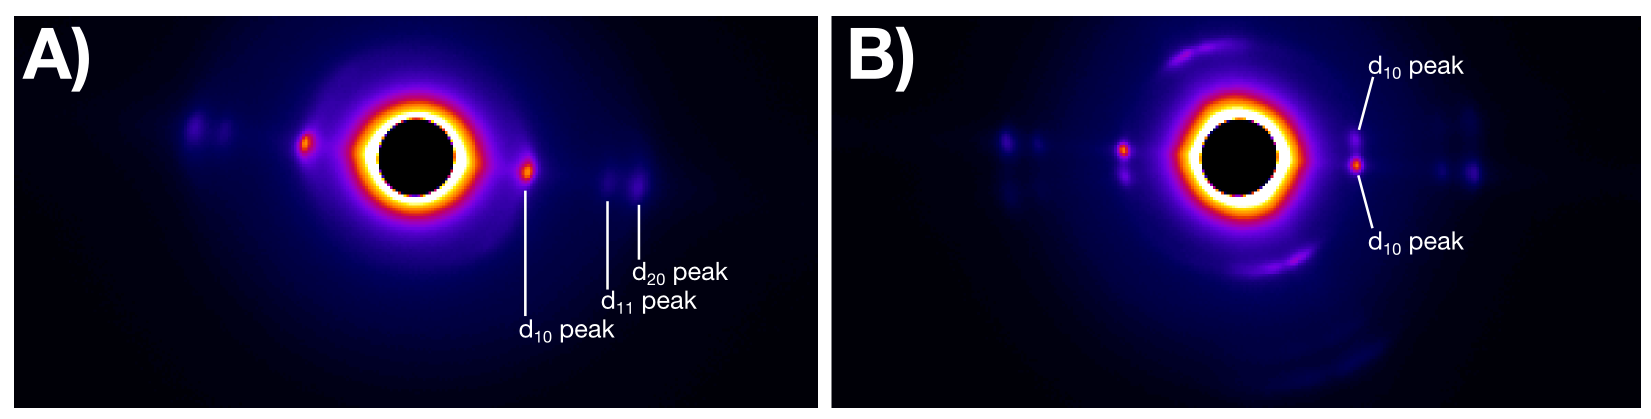
\includegraphics[width=.8\linewidth]{figures/x_ray_image_montage}
  \caption{\label{fig:imgs}
  	X-ray diffraction images.
    A) An X-ray diffraction image exhibits $d_{10}$, $d_{11}$, and
    $d_{20}$ peaks; the first and last are proportional to the
    distance between adjacent rows of thick filaments. B) In this
    image, two fibers at slight angles to each other have generated
    multiple $d_{10}$ peaks which must be segregated during the
    detection process. Such two-fiber exposures occur rarely in the 
    test corpus used in this work and are successfully processed by 
    the automated grouping of peaks. 
	}
	\vspace{-10pt}
\end{figure}
}

\newcommand{\figureworkflow}{
\begin{figure}[tbp]
  \centering
  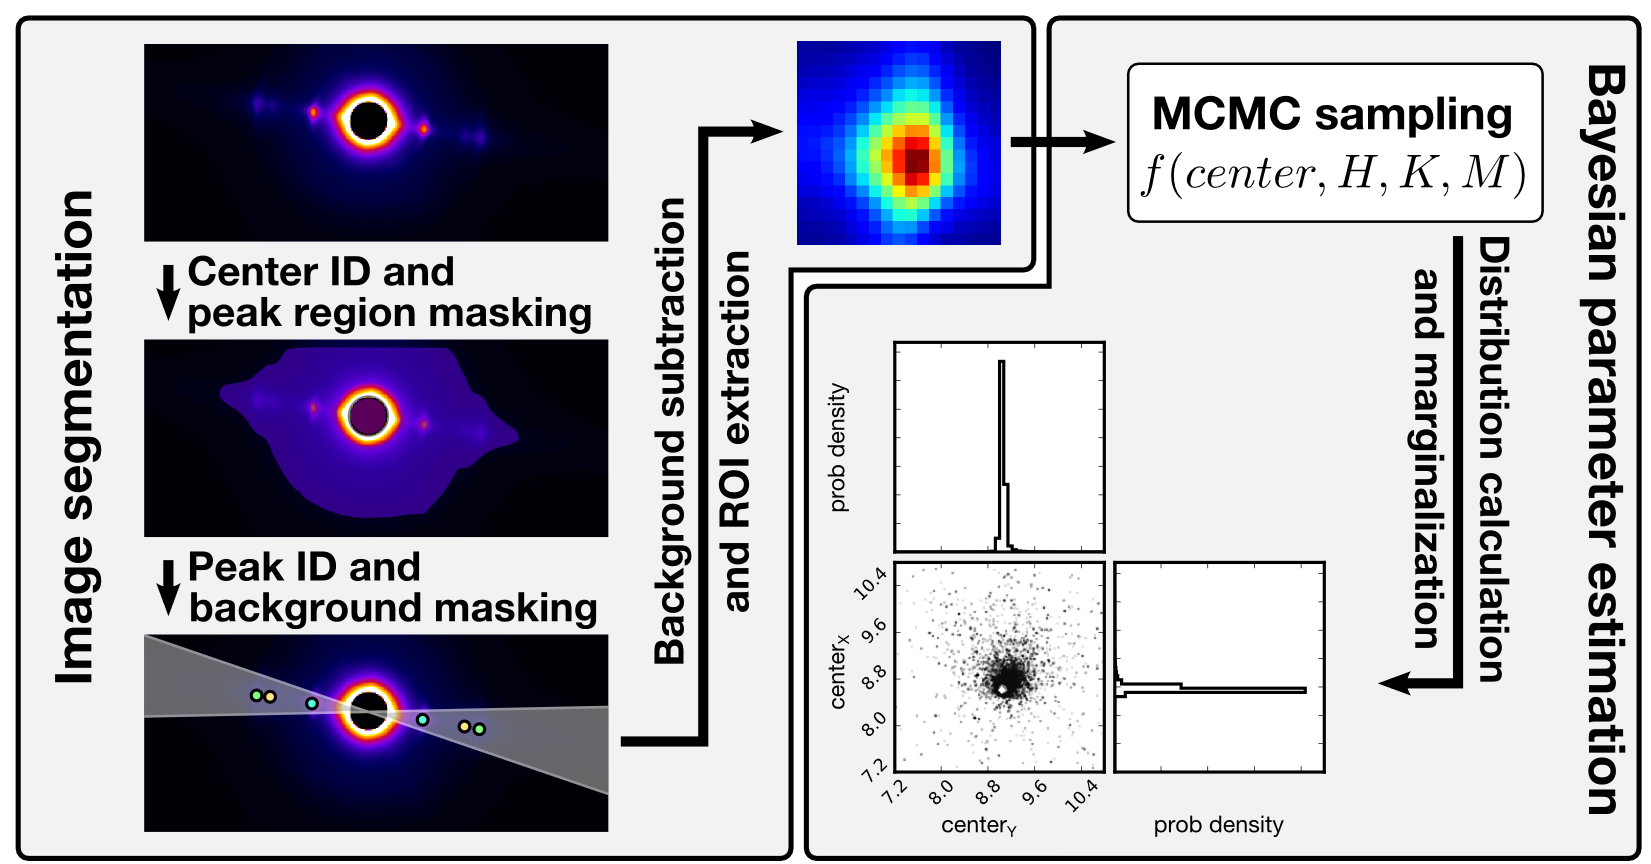
\includegraphics[width=\linewidth]{figures/img_analysis}
  \caption{\label{fig:workflow}
  	Analysis workflow.
    A) An X-ray diffraction image is read in. B) The blocked center
    region (in green) is detected and used as a landmark.  Low signal
    regions, the central blocked region, and image edges are masked
    off, leaving only the foreground outlined in white. C) The image
    is smoothed and peaks are detected, paired, and classified. To
    remove the exponentially decaying background from the peaks we
    mask off the area around the diffraction lines, shown in gray. The
    remaining background is then collapsed into a radial profile
    centered at the mean peak position.  A double exponential fit to
    this profile is computed and subtracted from the regions of
    interest surrounding the $d_{10}$ peaks, leaving just the peak
    signal shown in D).  E) We use an MCMC sampler to calculate the
    parameters generating the distributions these peaks are sampled
    from. F) We marginalize across peak parameters other than those of
    interest, extracting peak positions and the error in those
    position estimations.  
	}
	\vspace{-10pt}
\end{figure}
}

\newcommand{\figureerror}{
\begin{figure}[tbp]
  \centering
  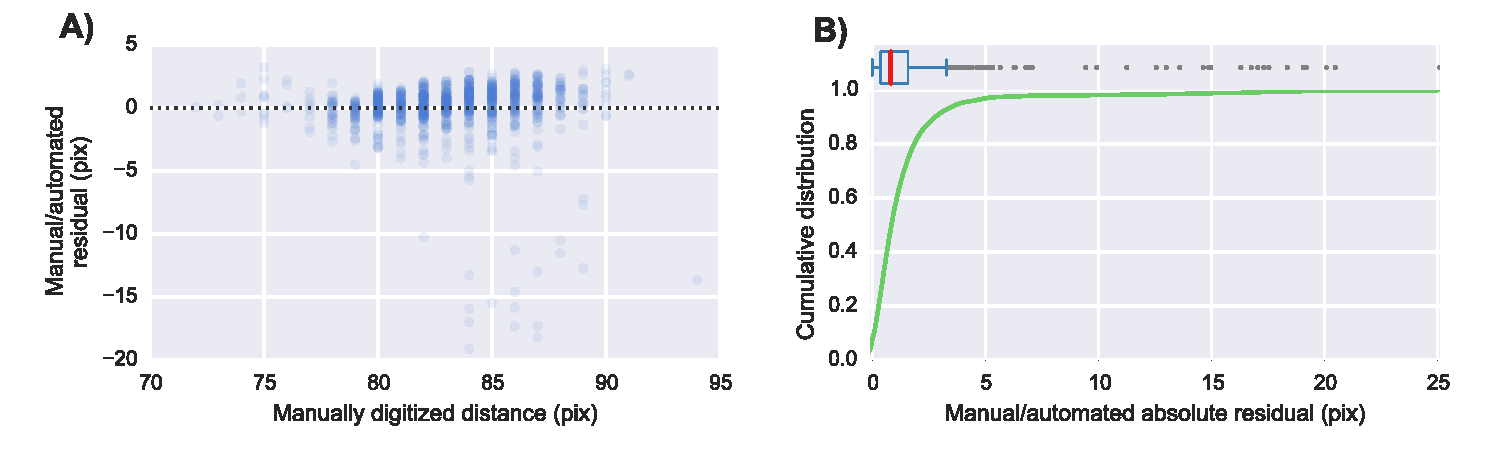
\includegraphics[width=\linewidth]{figures/hand_vs_auto}
  \caption{\label{fig:error}
  	Validation against hand-measurement. 
    A) The majority of residuals (between the manually and
    automatically measured $d_{10}$ peak distances) are within a
    single pixel of the manually digitized validation values. In a
    handful of outliers the automated method mis-identifies a closer
    structure as the $d_{10}$ pair. B) The cumulative distribution of
    the residuals shows that half of the automated measurements agree
    within 0.8 pixels and over 90\% agree within 3 pixels. A quartile
    box plot above shows the heavily left-weighted asymmetry of the
    residual distribution.  
    }
	\vspace{-10pt}
\end{figure}
}

\begin{document}


%%%%%%%%%%%
\frontmatter
\pagestyle{headings}  % switches on printing of running heads
\addtocmark{MCMC Analysis of X-ray Diffraction Images} % additional mark in the TOC


%%%%%%%%%%%
\mainmatter
\title{Automated Analysis of Muscle X-ray Diffraction \\ Imaging with MCMC}
\author{C.\ David Williams\inst{1} \and Magdalena Balazinska\inst{1} \and Thomas L.\ Daniel\inst{1}}
\institute{University of Washington, Seattle WA 98195, USA, \\
  \email{cdave@uw.edu}
  }
\maketitle


%%%%%%%%%%%
\begin{abstract}

  High-speed X-ray diffraction is the state-of-the-art approach to
  understanding protein structure and dynamics in living tissues,
  especially muscles.  Existing analytic approaches, however, require
  expert hand-digitization to extract parameters of interest. This
  produces repeatable measurements, but remains subjective and does
  not offer information on the precision of the measured parameters or
  strict reproducibility of analyzed data.  We developed a processing
  tool chain, which first segments the diffraction image into regions
  of interest using highly conserved features and then samples the
  possible parameter values with a Markov chain Monte Carlo approach.
  Our approach produces an automated, reproducible, objective estimate
  of relevant image parameters.
  \keywords{image analysis, X-ray diffraction, muscle structure, MCMC modeling}
\end{abstract}


%%%%%%%%%%%
\section{Motivation}
\label{sec:motivation}


The molecular regulation of force generating protein systems remains a
fundamental open problem in biology. Muscle uses a highly organized
lattice of interacting elastic and force generating molecules to
create controlled macro-scale movement \cite{Reedy1965,Millman1998}.
The advent of advanced X-ray diffraction imaging lets us analyze
protein motions at spatial and temporal scales never previously
realized, giving novel insight into the molecular basis of motion in
living systems.  

Exploring the dynamics of protein interactions in muscle requires
imaging that provides information at the nanometer to Angstrom scale.
X-ray diffraction provides that information and is unique in its
ability to image live muscle during movement, where other techniques
(e.g.\ solution biochemistry or cryo electron microscopy) are only able
to resolve properties of isolated individual molecular motors or
anatomic features of static, dried muscle. This ability to image
\textit{in vivo} makes X-ray diffraction the only direct means of
measuring the structural changes that generate force; all other
techniques that permit some level of molecular motor activity require
the removal of those motors from the regulating structure of the
thick/thin filament lattice and are thus less informative about the
processes that actually control activation.  This is a key advantage
of X-ray diffraction: changes in muscle microstructure are highly
correlated with changes in force production and any attempt to
separate the two removes significant aspects of the system's response
to real-world stimuli \cite{BrennerYu1985,Bagni1994}.

Surprisingly, we still use human experts to manually extract
structural parameters from X-ray images with NIH ImageJ via manual
selection of peaks and rock-of-eye parameter fitting. This produces
repeatable measurements but is subjective, fails to provide confidence
intervals for the measured values, and is not reproducible by naive
digitizers. Additionally hand digitization is a time-intensive
analytic technique, with a single digitizer able to process only a few
hundreds of images a day.  Historically this rate has been sufficient,
but new high-speed imaging systems let us investigate short-timescale
components of muscle contraction and generate data sets with many
thousands of images. The need for an automated and reproducible image
analysis tool chain is clear. 

\figurerig

We seek to build a service for the automated analysis of muscle
structure X-ray images. Users should specify the analysis they need
using a declarative query interface and the system should
automatically process the user's image database. In this work, we
present the first components of the processing tool chain at the heart
of this service. The toolchain first segments the
diffraction image into regions of interest using conserved features
and then samples the possible parameter values with a Markov chain
Monte Carlo approach.


%%%%%%%%%%%
\section{Prototype}
\label{sec:proto}


We focus initially on measuring the $d_{10}$ parameter, a crucial
spacing in muscle shown in Figures~\ref{fig:rig} and \ref{fig:imgs}.
The $d_{10}$ spacing determines the distance which muscle's molecular
motors must bridge in order to bind and generate force
\cite{Williams2013}. This distance changes during contraction and thus
regulates the force produced \cite{George2013}.

Images generated during experiments share several key features, which
serve as challenges or fiduciary marks during analysis. As seen in
Figure~\ref{fig:imgs}, the brightest part of the image background is
occluded by a circular stop. This physical block prevents damage to
the detector from the high photon flux at the center of the X-ray
beam. Surrounding the blocked region, the remainder of the image
displays an exponentially decaying background. We must locate and
model the symmetric pairs of diffraction peaks interrupting the
exponential background. Our core data analysis pipeline includes two
steps: image segmentation and image modeling with MCMC processes.

\figureimgs

\subsection{Image segmentation}
\label{subsec:imgseg}

The system first identifies the dark central circular blocked region
to act as a relative landmark for subsequent operations. Consistent
with experimental design, we assume it contains the center of the
diffraction pattern. The edge of the background surrounding the block
is the brightest region, so the system first splits the image between
areas with values less than and greater than two standard deviations
above the mean. This partitioning yields a binary image where the
center blocked region is surrounded by a halo of the upper end of the
pattern background and occasional dots where diffraction peaks rise
more than two standard deviations above background. We convert this
binary image to a hierarchical contour set with OpenCV, an open source
library of standard image processing techniques \cite{opencv}. We then
take the blocked region to be the inner-most contour and model it as
the smallest enclosing circle, shown as light green in
Figure~\ref{fig:workflow}B. 

With the central blocked region located, we identify local maxima in
three by three groups after Gaussian smoothing with kernel having a
three pixel standard deviation. We reject resulting maxima in regions
unlikely to provide peaks of interest before attempting to match peak
pairs. Masked rejection-regions consist of: 1) a circular zone around
the central blocked region where the blocking generates non-peak local
maxima, 2) areas below the 80th percentile where detector noise
dominates, 3) areas near the image edge where peaks are partially
cropped. The resulting unmasked area from which we keep maxima is
bounded by a white border in Figure~\ref{fig:workflow}B.

\figureworkflow

Next, we cluster maxima into peak pairs based on their distance and
angle from the center of the blocked region. Starting with those
maxima nearest the blocked region, a corresponding maximum is sought
an equal distance away from the blocked region and located so that the
angle formed by the two maxima and the center of the blocked region is
180$^\circ$. In cases where the matching maxima is clipped by the
image frame or fails to be distinguished from background the initial
maximum is discarded. For a maxima to be considered a match its
distance and angle must match those of the initial maxima within 10\%.
With peak pairs now identified (shown as color matched dots in
Figure~\ref{fig:workflow}C), the diffraction center is identified by
taking the mean location between peak pairs and the background is
removed. 

We subtract the background by first masking arcs encompassing peak
pairs and then fitting a double exponential to a radial profile of the
remaining image. An arc swept 12$^\circ$ out on either side of each
peak pair masks the effect of the diffraction peaks on the background
(shown as a light gray arc under the peak pairs in
Figure~\ref{fig:workflow}C). We calculate a radial profile of the image
around the pattern center, omitting diffraction line regions. We fit a
double exponential function of the form $background = a+ b e^{-x c} +
d e^{-x e}$ to the radial profile. From these parameters we generate
an estimated background image and subtract it from the real image,
allowing us to extract the $d_{10}$ peaks as regions of interest (ROIs)
unhindered by an overlaid diffraction background.

\subsection{Image modeling with MCMC processes}
\label{subsec:modelmcmc}

With the background subtracted and the $d_{10}$ peaks identified and
isolated from the rest of the image as ROIs, we apply Markov chain
Monte Carlo (MCMC) sampling to determine the probability distributions
from which the peak parameters could be drawn. We treat the peaks as
being drawn from an underlying Pearson VII distribution, commonly used
to fit X-ray diffraction peaks \cite{Hall1977}. This process allows us
to generate possible peak matches using five parameters: peak center
x-location, peak center y-location, peak height, peak spread, and peak
decay rate.  We perform an initial peak fitting by residual
minimization between a generated peak and the extracted ROI. This
gives a set of starting parameters that we use, with random variation,
to initialize the positions of the MCMC agents that will explore the
model space. 

Before MCMC sampling we must define our query's likelihood and prior.
We choose a flat prior as our initial information about the model is
minimal. To calculate the likelihood we represent each pixel's photon
count as a Poisson process in the form $P(d|m)=e^{-m}
\left(m^{d}/d!\right)$ where $m$ is the model value and $d$ is the
experimental data value. These functions are fed into \textit{emcee},
an efficient MCMC analysis Python library \cite{ForemanMackey2013}.
After a burn in period of 100 steps, the sampler histories are erased
and a further 1000 steps are run to generate the posterior probability
distributions of our peak parameters. 

One of MCMC modeling's convenient features is that extracting only a
subset of parameters marginalizes across those we discard. That is,
when we are interested in only the x- and y-locations of the peak
center to precisely calculate $d_{10}$ spacing (as in
Figure~\ref{fig:workflow}F), we automatically integrate our uncertainty
about peak height, spread, and decay.


%%%%%%%%%%%
\section{Preliminary Evaluation}
\label{sec:eval}


We apply our workflow to a test corpus of 1,220 images generated using
X-ray diffraction during insect flight muscle research at the Argonne
National Laboratory BioCAT Beamline. Sample high-quality and
challenging images are shown in Figures~\ref{fig:imgs}A and
\ref{fig:imgs}B \cite{Irving2006}. We tested the output of our
automated system against the results from a domain expert manually
digitizing peak locations. Our initial image segmentation step,
described in Section~\ref{subsec:imgseg}, successfully identifies the
center blocked region of each image in greater than 99\% of images in
our test corpus. The overall process allows us to calculate
peak-to-peak distances to sub-pixel accuracy with a confidence
interval of 90\%, with residuals between expectation values and
manually digitized peak positions shown in Figure~\ref{fig:error}.
MCMC sampling combined with image segmentation allows us to precisely,
accurately, and automatically locate the $d_{10}$ peak centers and
thus calculate the lattice spacing measured by a diffraction image to
within 0.03 nm.

\figureerror

Because the images in our corpus are a standard sample of those
produced by high-speed X-ray diffraction, our positive preliminary
results are a strong indication for the potential of this approach.


%%%%%%%%%%%
\section{Challenges and Next Steps}
\label{sec:challenges}

Our initial data processing pipeline produces an automated,
reproducible, objective estimate of relevant image parameters but the
following challenges remain:

\begin{itemize}
\item Development of a declarative language to describe processing
    steps will speed use of this technique and ease reproducibility.
    The key question is to define the types of operations that users
    should be able to specify and how to specify them. Our goal is to
    generalize to a broad set of analysis needs for X-ray images of
    muscle structure.
\item Packaging of this tool chain into a cloud deployable
    containerized image will enable trivial scaling to work with
    larger datasets. Furthermore, the ability to access to tool chain
    directly through a web browser with automatic back-end deployment
    of the analysis pipeline will facilitate adoption. 
\item This toolchain works best when applied to sharp and well defined
    images produced by isolated fibers. When working with images
    produced by \textit{in vivo} samples, such as those taken through
    a fly thorax, diffraction from multiple muscles in different
    orientations is common. These multiple-muscle images produce a
    more extreme version of the image shown in Figure~\ref{fig:imgs}B,
    where twin rotated peaks that are twisted and blurred about the
    center of the diffraction pattern and may have substantially
    divergent $d_{10}$ distances. Twin rotated peaks must be classified by
    diffraction line/muscle and treated independently during analysis. 
\item Application of these techniques to coming ultra-high
    temporal-resolution images with far lower signal:noise will strain
    autosegmentation and peak-fitting techniques. 
\end{itemize}

The increasing prevalence of advanced diffractive imaging techniques
demands data analytic methods that can handle, objectively and
reproducible, significant increases in the volume of data generated
and analyzed. This toolchain is a first step in a process that will
greatly increase the power and capabilities of a widely used approach
to understanding protein structure in living tissue. 

%%%%%%%%%%%
\section{Acknowledgments}
\label{sec:acknowledgments}

This work was supported in part by NSF grant IIS-1110370, the Intel
Science and Technology Center for Big Data, the Army Research Office
through ARO Grants W911NF-13-1-0435 and W911NF-14-1-0396, an award
from the Gordon and Betty Moore Foundation and the Alfred P Sloan
Foundation, the Washington Research Foundation Fund for Innovation in
Data-Intensive Discovery, and the UW eScience Institute.

We thank Jake VanderPlas for helpful discussions of statistical
techniques, Tom Irving for advice on X-ray imaging, Gideon Dunster for
digitization of diffraction images, and Simon Sponberg for the sharing
of diffraction images. 


\scriptsize
\bibliography{articles,paper}
\bibliographystyle{abbrv}

\end{document}
